\newcommand{\tax}{\textsf{t\_ax}}
\newcommand{\tpi}{\textsf{t\_pi}~}
\newcommand{\tlam}{\textsf{t\_lam}~}
\newcommand{\tapp}{\textsf{t\_app}~}
\newcommand{\ptc}{\textsf{p\_tc}}

\newcommand{\rall}{\textsf{r\_all}}
\newcommand{\rarr}{\textsf{r\_arr}}
\newcommand{\rapp}{\textsf{r\_app}}
\newcommand{\rtapp}{\textsf{r\_App}}
\newcommand{\rlam}{\textsf{r\_lam}}
\newcommand{\rtlam}{\textsf{r\_Lam}}

\newcommand{\D}{\mathcal{D}}

\newcommand{\bc}[2]{\ensuremath{[\,#1\,\vdash #2\,]}}

The programming and proof environment Beluga~\cite{Pientka:IJCAR10,Pientka:FLOPS10,Pientka:CADE15} is another system that supports HOAS.
Object languages are encoded in the logical framework LF~\cite{Harper93jacm}, while proofs about these are expressed as total programs in contextual modal type theory, Beluga's reasoning logic.
The programs analyse LF derivation trees using pattern matching and higher-order unification.
In Beluga it is necessary to give the programs, or proof terms, explicitly, which are then proof checked as part of the type checker at compile time.
This stands in contrast to Coq and Abella, both of which are interactive systems with a tactic language for proof term construction.

The biggest difference, however, lies with Beluga's treatment of object level variables.
In particular, at the outermost level, there is no such thing as a free object variable.
This is in stark contrast to Coq's dangling de Bruijn indices and Abella's global nominal constants.
In Beluga we instead deal with \emph{contextual objects}, written $\bc{\Gamma}{K}$, that is objects $K$ (like types, terms, typing derivations) paired with contexts $\Gamma$ in which they are meaningful~\cite{Nanevski:ICML05,Pientka:POPL08}.

A an example consider the function type $X \to X$ where $X$ is a free type variable.
This function type is ill-formed under the empty type variable context $\Delta = \emptyset$.
In Coq and Abella we can express this type, as $0_\ty \to 0_\ty$ and respectively $n_0 \to n_0$, and then prove that assuming well-formedness entails absurdity, $\istyF{0}{0_\ty \to 0_\ty} \implies \bot$ and $\aj{\emptyctx}{\istyFh{n_0 \to n_0}} \implies \bot$.
Meanwhile in Beluga, we observe that the contextual object $\bc{\emptyctx}{x \to x}$ is not even syntactically well-formed, since $x \notin \emptyctx$.
An immediate consequence of this is that the type formation judgement for F, which ensures that the context is covering all free type variables, becomes redundant.
Beluga's definition of F is obtained from Fig.~\ref{fig:sys-f-abella} by removing all references to type formation.
The definition of \SysL is identical to the one for Abella (Fig.\ref{fig:sys-l-abella}).

Recall that context management was completely manual in Coq.
Each judgement required well-chosen generalisations and custom invariants to accurately track contextual information.
In Abella the situation was noticeably better, as contexts at the object level were kept implicit and handled by the system.
At the reasoning level they did, however, surface as explicit, unstructured sequences of judgements.
The desired contextual structure then had to be imposed with auxiliary predicates, together with copious amounts of inversion lemmas.

Beluga contexts, on the other hand, are sequence of not necessarily homogeneous declarations.
Each declaration can depend on prior declarations and encapsulate multiple pieces of related information using a dependent record.
Contexts are first class citizens and \emph{context schema} ascription, $\Gamma \OF S$, is used to ensure that $\Gamma$ satisfies certain structural constraints.

Schemas are Beluga's main device to enforce invariants on contextual information.
The following allows us to prove propagation for \SysL.
\begin{align*}
  S_{\lambda W} \eqdef [x\of\TmL \mrel{;} \typingLh{x}{\Prp}] \mrel{+} [x\of\TmL \mrel{;} \typingLh{x}{a} \mrel{;} \typingLh{a}{\Prp}]
\end{align*}

Note how it separates PTS variables into type and term variables via the associated typing information, which already imposes the necessary semantic contextual information.
The prove of propagation for \SysL is then straightforward.\footnote{Surprisingly this is the only language local property required for the Beluga proof.}
We simply implement a total recursive function of the following type:
\begin{align*}
  \mAll{\Gamma \of S_{\lambda W}} \bc{\Gamma}{\typingLh{a}{b}} \implies \bc{\Gamma}{\mathsf{type\_correct}\,b}
\end{align*}

The contextual predicate $\bc{\Gamma}{\mathsf{type\_correct}\,b}$ encodes that $b$ is either $\Typ$ or it can be typed with some sort $s$.
We pattern match $\D \OF \bc{\Gamma}{\typingLh{a}{b}}$ and obtain seven cases.
The first four are structural, recursively descending into sub-derivations.
The only part that is non-obvious is the traversal of binders, where various pieces of information are added to the context.
These have to be packaged into declaration blocks in order to satisfy $S_{\lambda W}$.
More interesting though are the three base cases.
When we compare the matched type against $S_{\lambda W}$, we observe three ways in which $\D$ could have been obtained from the context.
The first and third are trivial as they unify $b$ with $\Prp$ which can be typed with the sort $\Typ$.
For the remaining case we know that $b$ can be typed with the sort $\Prp$,  contextual information that was packaged together with the matched judgement.
Note that throughout the construction we exploit that Beluga natively supports substitution into parametric sub-derivations.

At this point we are able to constructed our third equivalence proof.
The definitions of $\tyr$ and $\tmr$ exactly coincide with Abella.
We are going to primarily concern ourselves with the schemas, which best illustrate Beluga's tracking of contextual information.

{\color{red} -- MARK --}

Since Beluga does not natively provide equality, we also define three LF types that encode equality of the various syntactic sorts, each with a single reflexive constructor.

We begin with the functionality of $\tyr$, that is, we implement a recursive function of type
\begin{align*}
  \mAll{\Gamma \of S_{\tyr}} \bc{\Gamma}{A \tyr a} \implies \bc{\Gamma}{A \tyr a'} \implies \bc{\Gamma}{a =_{\lambda} a'},
\end{align*}
where
\begin{align*}
  S_{\tyr} \eqdef [y \of \TmL] \mrel{+} [x\of\TyF \mrel{;} y\of\TmL \mrel{;} h\of x \tyr y]
\end{align*}
The context schema expresses the tightest invariant that holds about the rules defining the $\tyr$ relation.% on page \pageref{rel-rules}.
In particular, we may either introduce a $\TmL$ variable in the rule \rarr~or we introduce a $\TyF$ variable $x$ and a $\TmL$ variable $y$ together with $x \tyr y$ in the rule \rall.

We go over the definition of this function in detail to illustrate how contextual information is generated and processed when binders are traversed.
At a high level, the proof is by induction on the derivation of $d_1 \OF \bc{\Gamma}{A \tyr a}$ and pattern matching on $d_2 \OF \bc{\Gamma}{A \tyr a'}$.
We have to cover three cases, two structural and one for a context extraction.

Let $d_1$ be a derivation that ends in the rule \rarr, i.e.~ is $A = B \to C$ and $a = \Prod{b}c$ for some $B,C,b,c$. Then $d_1 = \bc{\Gamma}{\rarr~\D_{11}~\D_{12}}$ where
we have sub-derivations $\D_{11} \OF \bc{\Gamma}{B \tyr b}$ and $\D_{12} \OF \bc{\Gamma, y \of \TmL}{C \tyr \lpApp{c}{y}}$.
As a consequence, $d_2$ must have also ended with the \rarr~rule. This is accomplished by pattern matching on $d_2 = \bc{\Gamma}{\rarr~\D_{21}~\D_{22}}$. Hence $a' = \Prod{b'}c'$, with sub-derivations $\D_{21} \OF \bc{\Gamma}{B \tyr b'}$ and $\D_{22} \OF \bc{\Gamma, [y \of \TmL]}{C \tyr \lpApp{c'}{y}}$.
We have to prove that $\Prod{b}c =_{\lambda} \Prod{b'}c'$, which is only possible if we can unify $b$ with $b'$ and $c$ with $c'$.
This is easily achieved through invocations of the inductive hypothesis on $\bc{\Gamma}{\D_{11}}$ and $\bc{\Gamma}{\D_{21}}$ and, respectively, on $\bc{\Gamma}{\D_{12}}$ and $\bc{\Gamma}{\D_{22}}$.

Next we consider the \rall~rule. By pattern matching on $d_1$ with $\bc{\Gamma}{\rall~\lambda x.\lambda u.\D_1}$ we obtain $A = \All B$, $a = \Prod{\Prp} b$,
and $\D_1$ stands for $\bc{\Gamma, x \of \TyF, y \of \TmL, h \of x \tyr y}{\lpApp{B}{x} \tyr \lpApp{b}{y}}$.
Similarly, by pattern matching on $d_2$ with $\bc{\Gamma}{\rall~\lambda x.\lambda u.\D_2}$ we learn $a' = \Prod{\Prp} b'$ and $\D_2$ stands for
$\bc{\Gamma, x \of \TyF, y \of \TmL, h \of x \tyr y}{\lpApp{B}{x} \tyr \lpApp{b'}{y}}$.
%
To apply the induction hypothesis, we also must ensure that the context invariant is satisfied. We hence pack the assumptions $ x \of \TyF, y \of \TmL, h \of x \tyr y$ in a dependent record $r$ and
invoke the induction hypothesis on $\bc{\Gamma, r}{\lpApp{\D_1}{r_x,r_y,r_h}}$ and $\bc{\Gamma, r}{\lpApp{\D_2}{r_x,r_y,r_h}}$. We rely on the built-in simultaneous substitution operation to replace $x$ with the projection $r_x$, $y$ with the projection $r_y$, and $h$ with the projection $r_h$. By uncurrying the LF functions denoting parametric and hypothetical derivations, we can enforce the stated context invariant which guarantees naturally that whenever we have a $\TyF$ variable $x$, we also must have a related  $\TmL$ variable $y$ (and vice versa).

% The scenario is similar for $d_{21}$.
% That is, we cannot directly apply our inductive hypothesis to unify $b$ and $b'$.


Finally, we consider the variable case where we extract a declaration from the context. The derivation $d_1$ must have come from a block of the form $r \OF [x\of\TyF \mrel{;} y\of\TmL \mrel{;} h \of x \tyr y]$, that is $d_1 = r_h$ and stands for a derivation
$\bc{\Gamma}{r_x \tyr r_y}$. Note that by assumption $d_2$ stands for $\bc{\Gamma}{r_x \tyr a'}$.  By pattern matching on $d_2$, $a'$ must be $r_y$, since assumptions in a context are unique.
We can use $S_{\tyr}$ to obtain injectivity of $\tyr$ in a similar fashion.
%
In contrast, to context relations that are commonly used in Abella and Coq, Beluga supports developing proofs by enforcing context invariants using context schemas. While in this example, we can directly derive the context invariant needed in the proof from the definitions of $\tyr$ and $\tmr$, this may not always be the case.  Instead, we may need to generalize. The contrast between the joint context in Beluga versus the relational context approach in Abella is also highlighted in \cite{Felty:ITP10,Felty:orbi-survey}.


To obtain functionality and injectivity of $\tmr$ we can follow a similar pattern, generalizing the previous context schema  to
\begin{align*}
  S_{\tmr} \eqdef [x\of\TmF \mrel{;} y\of\TmL \mrel{;} h\of x \tmr y] \mrel{+} [x\of\TyF \mrel{;} y\of\TmL \mrel{;} h\of x \tyr y]
\end{align*}
Again this schema can be derived from the definition of the $\tmr$ rules.
When we compare the two context schemas it should quickly be come apparent that any $\Gamma \of S_{\tmr}$ contains at least as much information as required by $S_{\tyr}$. We also note that while the rules $\tyr$ do only refer to $\tyr$ assumptions and not to $\tmr$ assumptions. Based on this dependency \cite{Virga99phd}, Beluga supports strengthening. In other words, if we need to appeal to functionality and injectivity of $\tyr$ within the proof of functionality and infjectivity of $\tmr$, we may strengthen the given context such that it satisfies $S_{\tyr}$, appeal to functionality and injectivity of $\tyr$, and the weaken the result to use it in the context satisfying $S_{\tmr}$ (see \cite{Felty:orbi-survey} for a detailled discussion especially in contrast to context relations).

% Beluga is capable of implicitly strengthening contexts in this way.
% So when the proof of functionality of $\tmr$ relies on the functionality of $\tyr$ we can directly pass the given complex context and do not need to invoke any stripping functions or strengthening lemmas beforehand.
% In other words, we get directly $\Gamma \of S_{\tyr}$ rather than $\mathsf{str}(\Gamma) \of S_{\tyr}$.
% The only other interesting aspect here than is the injectivity of $\tmr$ relies on $\tyr$ and $\tmr$ having disjoint ranges, which thanks to higher-order unification is very easy to obtain under contexts $\Gamma \of S_{\tmr}$.

When it comes to the totality and preservation results we define a predicate $\mathsf{exists\_rel\_prop}~A$ that succeeds, if there exists a type $A$ s.t. $A \tyr a$ and $\typingLh{a}{\Prp}$:
\begin{align*}
\inferrule*{A \tyr a \quad \typingLh{a}{\Prp}}{ \mathsf{exists\_rel\_prop}\,A}
%  \mathsf{exists\_rel\_prop}\,A \iff \mEx{a} A \tyr a \mAnd \typingLh{a}{\Prp}
\end{align*}
The result itself is then established with a function of type
\begin{align*}
  \mAll{\Gamma \of S_{\tyr W}^{\rightarrow}} \mAll{A \of \bc{\Gamma}{\TyF}} \bc{\Gamma}{\mathsf{exists\_rel\_prop}\,A}
\end{align*}
where $S_{\tyr W}$ extends the context schema $S_{\tyr}$ with additional typing information in each block:
\begin{align*}
  S_{\tyr W}^{\rightarrow} \eqdef [y\of\TmL \mrel{;} v\of\typingLh{y}{a}] \mrel{+} [x\of\TyF \mrel{;} y\of\TmL \mrel{;} h\of x \tyr y \mrel{;} v\of\typingLh{y}{\Prp}]
\end{align*}
%
We note that in Beluga we can directly induct on $A$ and we do not need to reify it as an inductive definition as in Abella. We are not going to present its construction in detail.
The interesting part is due to the fact that we cannot have an object level type formation judgement for Beluga's variant of F types.
The key part here is the typing $A \of \bc{\Gamma}{\TyF}$ which is itself contextual.
Since every type is well-formed by construction, we prove this result immediately by induction on $A$.
Recall that this was not possible in the Abella proof, where the well-formedness required a separate predicate that in turn was essential to carry the induction through.

For similar reasons the encoding of the goal for the inverse direction only yields
\begin{align*}
  \mathsf{exists\_rel\_type}\,a \iff \mEx{A} A \tyr a,
\end{align*}
that is, if there is some $A$ at all that is related via $\tyr$ then $A$ is well-formed by construction.
Interestingly, it appears that we need even more typing information in the left block of the schema in order to prove the respective Lemma:
\begin{align*}
  S_{\tyr W}^{\leftarrow} \eqdef &[y\of\TmL \mrel{;} v\of\typingLh{y}{a} \mrel{;} h\of A \tyr a \mrel{;} w \of \typingLh{a}{\Prp}]\\
  \mrel{+} &[x\of\TyF \mrel{;} y\of\TmL \mrel{;} h\of x \tyr y \mrel{;} v\of\typingLh{y}{\Prp}]
\end{align*}

The final two results are left and right preservation and totality of $\tmr$.
Both can be established with suitable encodings of the existentials and the following schema that interstingly works for both directions:
\begin{align*}
  S_{\tmr W} \eqdef &[x\of\TmF \mrel{;} y\of\TmL \mrel{;} h\of x \tmr y \mrel{;} u\of\typingFh{x}{A} \mrel{;} v\of\typingLh{y}{a} \mrel{;} j \of A \tyr a]\\
  \mrel{+} &[x\of\TyF \mrel{;} y\of\TmL \mrel{;} h\of x \tyr y \mrel{;} v\of\typingLh{y}{\Prp}]
\end{align*}

\begin{wrapfigure}{r}{0.3\textwidth}
% \begin{figure}[htb]
  \centering
\begin{minipage}{4.5cm}
  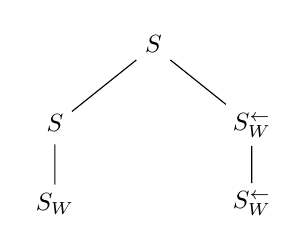
\begin{tikzpicture}
                [level/.style={sibling distance=25mm,
                               level distance=10mm}]
        \node [scale=0.9] (z){$S_{\tyr}$}
          child {node [scale=0.9] (a) {$S_{\tmr}$}
            child {node [scale=0.9] (a0) {$S_{\tmr W}$}}}
          child {node [scale=0.9] (b) {$S_W^{\leftarrow}$}
              child{node [scale=0.9] (d){$S_{\tyr W}^{\leftarrow}$}}};
%          \path (z) -- (a) node [midway] {$\leq$};
%          \path (z) -- (b) node [midway] {$\leq$};
              \end{tikzpicture}
  \end{minipage}
  \caption{Dependencies between Context Schemas}
  \label{fig:ctxschema}
\end{wrapfigure}
Once this schema has been fixed, constructing the two proofs is rather technical and lengthy, but not inherently different from the proofs in Coq or Abella.
Note that any $\Gamma \of S_{\tmr A}$ also matches both $S_{\tyr W}^{\rightarrow}$ and $S_{\tyr W}^{\leftarrow}$ so that corresponding results for type formation can easily be invoked.

In our proof development, we relied on different, but often related context schemas (invariants).
Compared to many existing benchmarks, this challenge problem exhibits a particularly rich context structure.
We describe the relationship between context schemas in Fig.~\ref{fig:ctxschema}. We can always weaken a context of schema $S_{\tyr}$ to any of the other schemas in the graph. Given our dependency graph of the different judgements (aka predicates), i.e.~$\tyr$, $\tmr$, etc., the graph also induces a strengthening relationship. We can always strengthen a context schema to pass it in place of a context that is higher in the hierarchy.






%%% Local Variables:
%%% mode: latex
%%% TeX-master: "fscd17"
%%% End:
